\documentclass[a4paper]{article}
\usepackage[a4paper,margin=0mm]{geometry}
\usepackage{fontspec}
\usepackage{unicode-math}
\usepackage{tikz}
\usetikzlibrary{calc}
\usepackage[table]{xcolor}
\usepackage[absolute]{textpos}
\usepackage{enumitem}
\usepackage{array}
\usepackage{multirow}

\setmainfont{Libertinus Serif}
\setsansfont{Libertinus Sans}
\setmathfont{Libertinus Math}

\definecolor{accent}{HTML}{0F6A52}
\definecolor{badge}{HTML}{A9CFC2}
\definecolor{ink}{HTML}{2A2E30}

\setlength{\TPHorizModule}{1mm}
\setlength{\TPVertModule}{1mm}
\setlength{\parindent}{0pt}
\pagestyle{empty}
\binoppenalty=10000 \relpenalty=10000

\newcommand{\LCOL}{16mm}
\newcommand{\RCOL}{111mm}
\newcommand{\COLW}{83mm}

\newcommand{\topicheader}[2]{%
\begin{textblock*}{194mm}(16mm,10mm)
\begin{tikzpicture}
\node[fill=accent,text=white,font=\sffamily\bfseries\fontsize{13}{13}\selectfont,
      minimum width=9mm,minimum height=9mm,inner sep=0pt] at (4.5mm,-4.5mm) {#1};
\node[font=\sffamily\bfseries\fontsize{15}{16}\selectfont,text=ink,anchor=west] at (12mm,-4.5mm) {#2};
\end{tikzpicture}
\end{textblock*}
\begin{textblock*}{194mm}(16mm,22.5mm)

\begin{tikzpicture}
\fill[accent] (0,0) rectangle (194mm,0.5mm);
\end{tikzpicture}
\end{textblock*}
}

\newcommand{\pagefooter}[1]{%
\begin{textblock*}{194mm}(8mm,286.41mm)
  
\begin{tikzpicture}
    \fill[accent] (0,0) rectangle (194mm,0.6mm);
  \end{tikzpicture}
\end{textblock*}
\begin{textblock*}{63.59mm}(8mm,288.27mm)
  {\sffamily\bfseries\color{accent}\fontsize{13}{16}\selectfont SAT 1200+}
\end{textblock*}
\begin{textblock*}{10mm}(188mm,288.27mm)
  \centering{\sffamily\color{accent}\fontsize{14}{16}\selectfont #1}
\end{textblock*}
}

\newcommand{\colrule}[2]{%
\begin{textblock*}{1mm}(105mm,#1mm)
\begin{tikzpicture}
\draw[black!65,line width=0.5pt] (0,0) -- (0,#2mm);
\end{tikzpicture}
\end{textblock*}
}

% Page kicker: left = module line, right = question range
\newcommand{\pagekicker}[2]{%
\begin{textblock*}{194mm}(16mm,25.2mm)
{\sffamily\bfseries\fontsize{10.5}{12}\selectfont\color{accent}#1}\hfill{\sffamily\fontsize{10}{12}\selectfont\color{black!70}#2}
\end{textblock*}
}

\setlength{\fboxsep}{1.4pt}
\setlength{\fboxrule}{0.5pt}
\newcommand{\pnum}[1]{\fcolorbox{ink}{white}{\sffamily\bfseries\fontsize{8}{8}\selectfont #1}~}

% centered display line inside a stem
\newcommand{\dsp}[1]{\par\vspace{1.4mm}\centerline{#1}\vspace{1.8mm}}

% student-produced response box
\newcommand{\gridbox}{%
\par\vspace{3mm}\noindent

\begin{tikzpicture}
\node[anchor=south west,font=\sffamily\bfseries\fontsize{7.5}{9}\selectfont,text=accent,inner sep=0pt] at (0,0.3mm) {STUDENT-PRODUCED RESPONSE};
\draw[ink,line width=0.7pt] (0,-9.5mm) rectangle (40mm,-0.8mm);
\node[anchor=west,font=\sffamily\fontsize{7.5}{9}\selectfont,text=black!55,inner sep=0pt] at (43mm,-5.2mm) {Write your answer in the box.};
\end{tikzpicture}\par}

\arrayrulecolor{accent}
\setlength{\arrayrulewidth}{0.7pt}
\renewcommand{\arraystretch}{1.35}

\newcommand{\figwrap}[1]{\par\vspace{2.5mm}\centerline{{\arrayrulecolor{ink}\setlength{\arrayrulewidth}{0.5pt}\renewcommand{\arraystretch}{1.3}#1}}\vspace{0.5mm}}

\begin{document}

% ================= PAGE 1: Mock Test 4 -- instructions + geometry reference sheet =================
\topicheader{4}{Mock Test 4}
\pagefooter{179}
\mbox{}%

\newcommand{\cardhead}[1]{{\sffamily\bfseries\color{accent}\fontsize{11.5}{14}\selectfont #1}\par\vspace{0.6mm}%
{\color{accent}\rule{\linewidth}{0.5pt}}\par\vspace{1.6mm}}
\newcommand{\bul}{\item[\textcolor{accent}{\rule[0.2mm]{1.5mm}{1.5mm}}]}

\begin{textblock*}{194mm}(16mm,28mm)
{\sffamily\bfseries\color{accent}\fontsize{26}{28}\selectfont Mock Test 4\par}
\vspace{1mm}
{\sffamily\color{ink}\fontsize{11}{14}\selectfont Full-length digital SAT Math practice \;\textperiodcentered\; 2 modules $\times$ 22 questions $\times$ 35 minutes\par}
\end{textblock*}

\begin{textblock*}{\COLW}(\LCOL,53mm)
{\fontsize{9.4}{12.2}\selectfont
\cardhead{How this test works}
\renewcommand{\arraystretch}{1.3}\setlength{\tabcolsep}{4pt}
\noindent\begin{tabular}{|>{\raggedright\arraybackslash}p{20mm}|>{\centering\arraybackslash}p{15mm}|>{\centering\arraybackslash}p{13mm}|>{\centering\arraybackslash}p{19mm}|}
\hline
\rowcolor{badge!55}\textbf{Module} & \textbf{Questions} & \textbf{Time} & \textbf{Calculator}\\\hline
Module 1 & 22 & 35 min & allowed\\\hline
Module 2 & 22 & 35 min & allowed\\\hline
\end{tabular}\par\vspace{2.2mm}
\begin{itemize}[leftmargin=5mm,itemsep=1.2mm,topsep=0mm,parsep=0mm]
\bul Time each module separately: 35 minutes, not a minute more. Rest for 5--10 minutes between the two modules.
\bul Use a calculator (the built-in Desmos graphing calculator or any approved calculator) on both modules.
\bul Module 1 is a standard mix of easy, medium and hard questions. Module 2 is the \emph{harder route} you reach by doing well on Module 1.
\bul Answer every question. There is no penalty for a wrong answer.
\bul Unless a problem says otherwise, all numbers are real, a function's domain is every real number for which it is defined, and figures are not necessarily drawn to scale.
\bul Do not look at any answers while you work. When you finish both modules, score yourself with the \textbf{Answer Sheets} section at the end of this book.
\end{itemize}
}
\end{textblock*}

\begin{textblock*}{\COLW}(\RCOL,53mm)
{\fontsize{9.4}{12.2}\selectfont
\cardhead{Student-produced responses (grid-ins)}
Some questions have no answer choices. Work out the answer and write it in the answer box (on the real test you type it in).
\begin{itemize}[leftmargin=5mm,itemsep=1.2mm,topsep=1.6mm,parsep=0mm]
\bul You may give an integer, a decimal, or a fraction. For one answer, $9/2$ and $4.5$ are both correct.
\bul Never enter a mixed number: write $7/2$ or $3.5$, not $3\,1/2$ (it would be read as $31/2$).
\bul Do not enter symbols or units such as \$, \%, or $\pi$. Enter the number only.
\bul An answer may use at most 5 characters (6 if it is negative), counting the slash and the decimal point.
\bul If an answer is a repeating decimal, enter it as a fraction such as $2/3$, or fill all the digits that fit: $0.6666$ or $0.6667$.
\bul If you find more than one correct answer, enter only one of them.
\end{itemize}
\vspace{1.2mm}
\noindent\fcolorbox{accent}{badge!25}{\parbox{\dimexpr\linewidth-2\fboxsep-2\fboxrule}{\centering\sffamily\fontsize{8.5}{11}\selectfont
\textbf{Example.} Answer $4\tfrac12$ \;$\rightarrow$\; enter \textbf{9/2} or \textbf{4.5}\par}}
\par\vspace{3mm}
\noindent{\sffamily\bfseries\color{accent}Pacing.}\ Q1--15: about 18 min. Q16--22: about 17 min. Keep the last 2--3 min for flagged questions and every blank grid-in (a blank is a guaranteed zero).
}
\end{textblock*}

% ---- Geometry reference sheet (full width card) ----
\begin{textblock*}{178mm}(16mm,156mm)
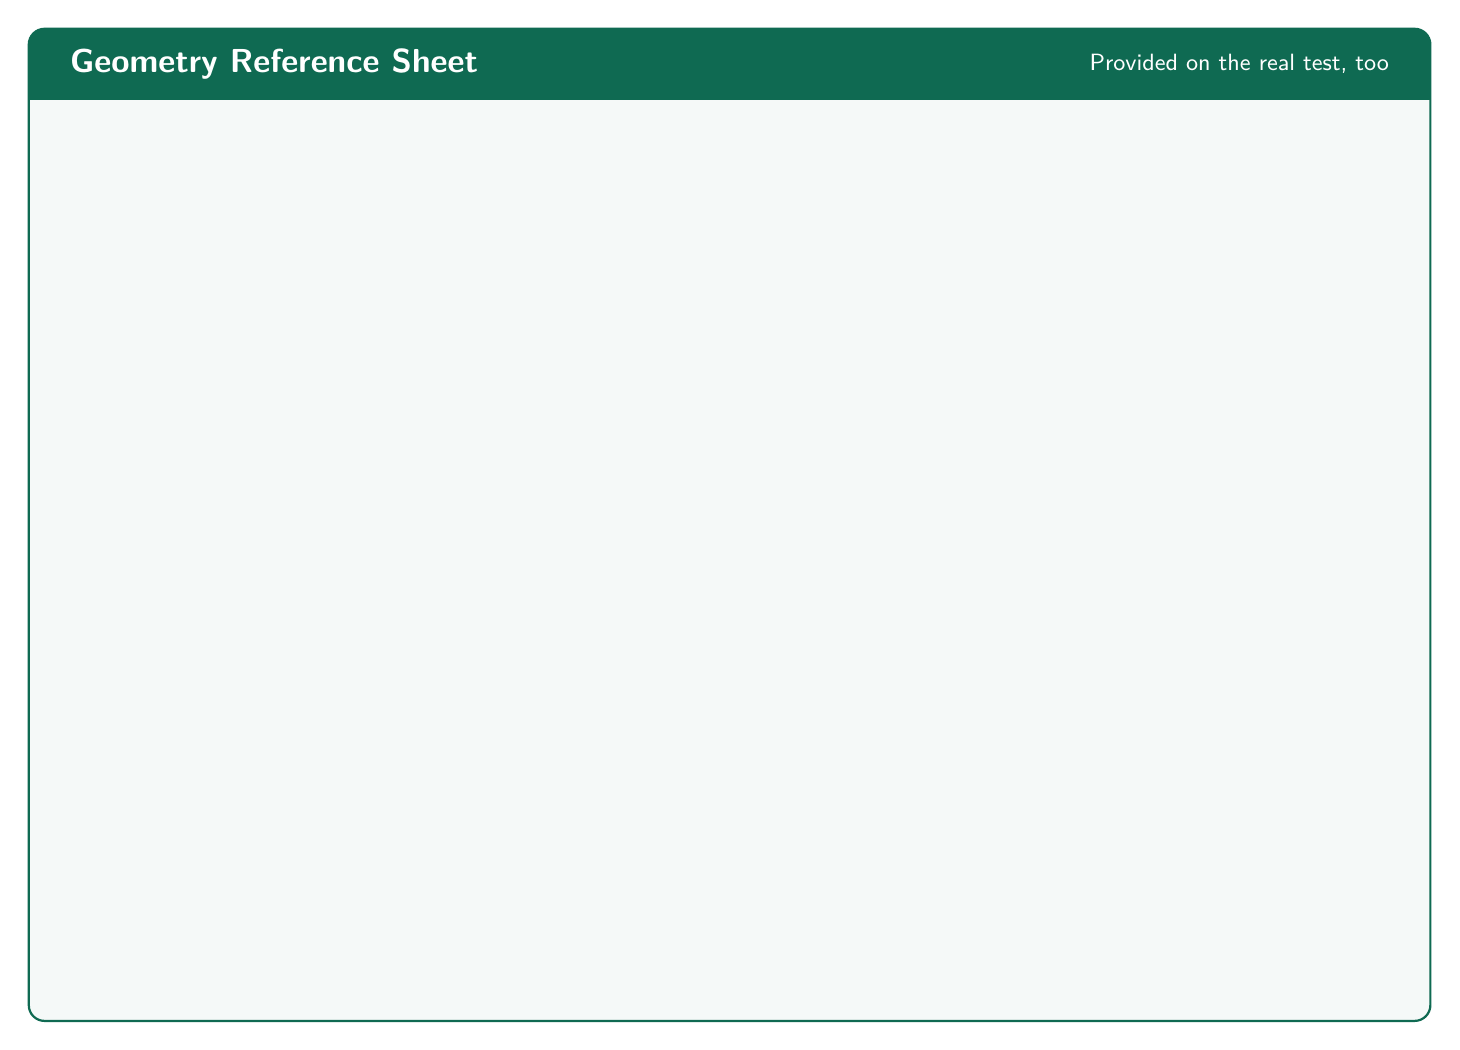
\begin{tikzpicture}
\draw[accent,line width=0.8pt,rounded corners=2mm,fill=badge!12] (0,0) rectangle (178mm,-126mm);
\fill[accent,rounded corners=2mm] (0,0) rectangle (178mm,-9mm);
\fill[accent] (0,-5mm) rectangle (178mm,-9mm);
\node[anchor=west,text=white,font=\sffamily\bfseries\fontsize{12}{14}\selectfont] at (4mm,-4.5mm) {Geometry Reference Sheet};
\node[anchor=east,text=white,font=\sffamily\fontsize{8.5}{10}\selectfont] at (174mm,-4.5mm) {Provided on the real test, too};
\end{tikzpicture}
\end{textblock*}

\newcommand{\refcell}[3]{\begin{textblock*}{42mm}(#1mm,#2mm)\begin{minipage}[t][36mm][t]{42mm}\centering #3\end{minipage}\end{textblock*}}
\newcommand{\refin}[2]{\parbox[b][26mm][b]{42mm}{\centering #1}\par\vspace{1.6mm}{\fontsize{9.6}{11.5}\selectfont #2}}
\tikzset{rf/.style={ink,line width=0.65pt},lb/.style={font=\fontsize{8.5}{9.5}\selectfont,inner sep=1.2pt}}

% ---------- row 1
\refcell{18}{167}{\refin{\begin{tikzpicture}[scale=1.25]
\draw[rf] (0,0) circle (9mm); \draw[rf] (0,0)--(9mm,0); \fill[ink] (0,0) circle (0.7pt);
\node[lb,above] at (4.5mm,0) {$r$};
\end{tikzpicture}}{Circle\\$A=\pi r^{2}$,\; $C=2\pi r$}}
\refcell{62}{167}{\refin{\begin{tikzpicture}[scale=1.25]
\draw[rf] (0,0) rectangle (22mm,12mm);
\node[lb,below] at (11mm,0) {$\ell$}; \node[lb,right] at (22mm,6mm) {$w$};
\end{tikzpicture}}{Rectangle\\$A=\ell w$}}
\refcell{106}{167}{\refin{\begin{tikzpicture}[scale=1.25]
\draw[rf] (0,0)--(22mm,0)--(7mm,13mm)--cycle;
\draw[rf,dashed] (7mm,0)--(7mm,13mm);
\draw[rf] (7mm,0)++(0,1.8mm)--++(1.8mm,0)--++(0,-1.8mm);
\node[lb,below] at (11mm,0) {$b$}; \node[lb,left] at (7mm,6.5mm) {$h$};
\end{tikzpicture}}{Triangle\\$A=\tfrac12 bh$}}
\refcell{150}{167}{\refin{\begin{tikzpicture}[scale=1.25]
\draw[rf] (0,0)--(18mm,0)--(0,12mm)--cycle;
\draw[rf] (0,1.8mm)--(1.8mm,1.8mm)--(1.8mm,0);
\node[lb,below] at (9mm,0) {$a$}; \node[lb,left] at (0,6mm) {$b$}; \node[lb,above right] at (9mm,6mm) {$c$};
\end{tikzpicture}}{Right triangle\\$c^{2}=a^{2}+b^{2}$}}

% ---------- row 2
\refcell{18}{204}{\refin{\begin{tikzpicture}[scale=1.25]
\draw[rf] (0,0)--(19.053mm,0)--(0,11mm)--cycle;
\draw[rf] (0,1.8mm)--(1.8mm,1.8mm)--(1.8mm,0);
\node[lb,below] at (9.5mm,0) {$x\sqrt3$}; \node[lb,left] at (0,5.5mm) {$x$}; \node[lb,above right] at (9.5mm,5.5mm) {$2x$};
\node[lb] at (14.6mm,1.9mm) {\fontsize{6.5}{7}\selectfont$30^\circ$}; \node[lb] at (3.2mm,8.2mm) {\fontsize{6.5}{7}\selectfont$60^\circ$};
\end{tikzpicture}}{$30^\circ$--$60^\circ$--$90^\circ$ triangle}}
\refcell{62}{204}{\refin{\begin{tikzpicture}[scale=1.25]
\draw[rf] (0,0)--(10mm,0)--(0,10mm)--cycle;
\draw[rf] (0,1.8mm)--(1.8mm,1.8mm)--(1.8mm,0);
\node[lb,below] at (5mm,0) {$s$}; \node[lb,left] at (0,5mm) {$s$}; \node[lb,above right] at (5mm,5mm) {$s\sqrt2$};
\end{tikzpicture}}{$45^\circ$--$45^\circ$--$90^\circ$ triangle}}
\refcell{106}{204}{\refin{\begin{tikzpicture}[scale=1.2]
\draw[rf] (0,0) rectangle (16mm,9mm);
\draw[rf] (16mm,9mm)--(22mm,13mm)--(6mm,13mm)--(0,9mm);
\draw[rf] (16mm,0)--(22mm,4mm)--(22mm,13mm);
\draw[rf,dashed] (6mm,13mm)--(6mm,4mm)--(22mm,4mm); \draw[rf,dashed] (0,0)--(6mm,4mm);
\node[lb,below] at (8mm,0) {$\ell$}; \node[lb,right] at (22mm,8.5mm) {$h$}; \node[lb,below right] at (19mm,2mm) {$w$};
\end{tikzpicture}}{Rectangular solid\\$V=\ell wh$}}
\refcell{150}{204}{\refin{\begin{tikzpicture}[scale=1.2]
\draw[rf] (0,2.2mm) ellipse (7mm and 2.2mm);
\draw[rf] (-7mm,2.2mm)--(-7mm,14mm); \draw[rf] (7mm,2.2mm)--(7mm,14mm);
\draw[rf] (0,14mm) ellipse (7mm and 2.2mm);
\draw[rf,dashed] (0,14mm)--(7mm,14mm); \fill[ink] (0,14mm) circle (0.6pt);
\node[lb,above] at (3.5mm,14mm) {$r$}; \node[lb,right] at (7mm,8mm) {$h$};
\end{tikzpicture}}{Right circular cylinder\\$V=\pi r^{2}h$}}

% ---------- row 3
\refcell{18}{241}{\refin{\begin{tikzpicture}[scale=1.15]
\draw[rf] (0,0) circle (10mm);
\draw[rf] (-10mm,0) arc (180:360:10mm and 2.8mm); \draw[rf,dashed] (-10mm,0) arc (180:0:10mm and 2.8mm);
\draw[rf] (0,0)--(10mm,0); \fill[ink] (0,0) circle (0.7pt); \node[lb,above] at (5mm,0) {$r$};
\end{tikzpicture}}{Sphere\\$V=\tfrac43\pi r^{3}$}}
\refcell{62}{241}{\refin{\begin{tikzpicture}[scale=1.2]
\draw[rf] (0,2.2mm) ellipse (7mm and 2.2mm);
\draw[rf] (-7mm,2.2mm)--(0,16mm)--(7mm,2.2mm);
\draw[rf,dashed] (0,16mm)--(0,2.2mm); \draw[rf,dashed] (0,2.2mm)--(7mm,2.2mm);
\fill[ink] (0,2.2mm) circle (0.6pt);
\node[lb,left] at (0,9.5mm) {$h$}; \node[lb,above] at (3.5mm,2.2mm) {$r$};
\end{tikzpicture}}{Right circular cone\\$V=\tfrac13\pi r^{2}h$}}
\refcell{106}{241}{\refin{\begin{tikzpicture}[scale=1.2]
\draw[rf] (0,0)--(16mm,0)--(22mm,4mm); \draw[rf] (0,0)--(10mm,15mm)--(16mm,0); \draw[rf] (10mm,15mm)--(22mm,4mm);
\draw[rf,dashed] (0,0)--(6mm,4mm)--(22mm,4mm); \draw[rf,dashed] (6mm,4mm)--(10mm,15mm);
\node[lb,below] at (8mm,0) {$\ell$}; \node[lb,below right] at (19mm,2mm) {$w$}; \node[lb,left] at (10mm,9.5mm) {$h$};
\end{tikzpicture}}{Rectangular pyramid\\$V=\tfrac13\ell wh$}}
\begin{textblock*}{40mm}(151mm,247mm)
{\fontsize{9.2}{12}\selectfont\raggedright
\textcolor{accent}{\rule[0.3mm]{1.6mm}{1.6mm}}\; A circle has 360 degrees of arc.\par\vspace{1.2mm}
\textcolor{accent}{\rule[0.3mm]{1.6mm}{1.6mm}}\; The angles of a triangle add up to 180 degrees.\par\vspace{1.2mm}
\textcolor{accent}{\rule[0.3mm]{1.6mm}{1.6mm}}\; $r$ radius, $\ell$ length, $w$ width, $b$ base, $h$ height.\par}
\end{textblock*}

\clearpage

% ===== Module 1, page 1 =====
\topicheader{4}{Mock Test 4}
\pagefooter{180}
\colrule{34}{236}
\mbox{}%
\pagekicker{Mock 4 \textperiodcentered{} Module 1 \textperiodcentered{} 22 questions \textperiodcentered{} 35 minutes}{Questions 1--8}
\begin{textblock*}{\COLW}(\LCOL,34mm)
{\fontsize{10.4}{13.4}\selectfont
\parbox[t][233mm][t]{\COLW}{%
\noindent\pnum{1} If $\dfrac{x}{4}+9=17$, what is the value of $x$?\par\vspace{2.2mm}
\hspace*{7mm}(A)\ $8$\\[1.8mm]
\hspace*{7mm}(B)\ $26$\\[1.8mm]
\hspace*{7mm}(C)\ $32$\\[1.8mm]
\hspace*{7mm}(D)\ $104$
\vfill

\noindent\pnum{2} The function $h$ is defined by $h(x)=x^{2}-5$. What is the value of $h(6)-h(2)$?\par\vspace{2.2mm}
\hspace*{7mm}(A)\ $11$\\[1.8mm]
\hspace*{7mm}(B)\ $30$\\[1.8mm]
\hspace*{7mm}(C)\ $31$\\[1.8mm]
\hspace*{7mm}(D)\ $32$
\vfill

\noindent\pnum{3} A recipe uses 3 cups of broth for every 2 cups of rice. How many cups of broth are needed for 14 cups of rice?\gridbox
\vfill

\noindent\pnum{4} A circular tabletop has an area of $81\pi$ square inches. What is the circumference, in inches, of the tabletop?\par\vspace{2.2mm}
\hspace*{7mm}(A)\ $9\pi$\\[1.8mm]
\hspace*{7mm}(B)\ $18\pi$\\[1.8mm]
\hspace*{7mm}(C)\ $36\pi$\\[1.8mm]
\hspace*{7mm}(D)\ $81\pi$
\vfill}}
\end{textblock*}
\begin{textblock*}{\COLW}(\RCOL,34mm)
{\fontsize{10.4}{13.4}\selectfont
\parbox[t][233mm][t]{\COLW}{%
\noindent\pnum{5} What is the slope of the line in the $xy$-plane with equation $4x-2y=10$?\par\vspace{2.2mm}
\hspace*{7mm}(A)\ $-5$\\[1.8mm]
\hspace*{7mm}(B)\ $-2$\\[1.8mm]
\hspace*{7mm}(C)\ $2$\\[1.8mm]
\hspace*{7mm}(D)\ $4$
\vfill

\noindent\pnum{6} Which of the following is a factor of $x^{2}+2x-24$?\par\vspace{2.2mm}
\hspace*{7mm}(A)\ $x-6$\\[1.8mm]
\hspace*{7mm}(B)\ $x-4$\\[1.8mm]
\hspace*{7mm}(C)\ $x+4$\\[1.8mm]
\hspace*{7mm}(D)\ $x+8$
\vfill

\noindent\pnum{7} In the $xy$-plane, a line has slope 3 and passes through the point $(2,5)$. The line crosses the $y$-axis at the point $(0,b)$. What is the value of $b$?\gridbox
\vfill

\noindent\pnum{8} A baker's sourdough starter doubles in mass every 6 hours. If the starter has a mass of 30 grams now, what will its mass be, in grams, 18 hours from now?\par\vspace{2.2mm}
\hspace*{7mm}(A)\ $60$\\[1.8mm]
\hspace*{7mm}(B)\ $90$\\[1.8mm]
\hspace*{7mm}(C)\ $240$\\[1.8mm]
\hspace*{7mm}(D)\ $540$
\vfill}}
\end{textblock*}
\clearpage

% ===== Module 1, page 2 =====
\topicheader{4}{Mock Test 4}
\pagefooter{181}
\colrule{34}{236}
\mbox{}%
\pagekicker{Mock 4 \textperiodcentered{} Module 1 \textperiodcentered{} 22 questions \textperiodcentered{} 35 minutes}{Questions 9--16}
\begin{textblock*}{\COLW}(\LCOL,34mm)
{\fontsize{10.4}{13.4}\selectfont
\parbox[t][233mm][t]{\COLW}{%
\noindent\pnum{9} A scatterplot of 40 vineyards shows the annual rainfall $x$, in inches, and the grape yield $y$, in tons per acre. The line of best fit passes through the points $(20,3.1)$ and $(36,4.7)$. According to the line of best fit, what is the predicted yield, in tons per acre, of a vineyard that receives 30 inches of rainfall?\par\vspace{2.2mm}
\hspace*{7mm}(A)\ $3.0$\\[1.8mm]
\hspace*{7mm}(B)\ $4.1$\\[1.8mm]
\hspace*{7mm}(C)\ $4.7$\\[1.8mm]
\hspace*{7mm}(D)\ $5.3$
\vfill

\noindent\pnum{10} A greenhouse uses large trays that hold 24 seedlings each and small trays that hold 15 seedlings each. A total of 40 trays hold 762 seedlings. How many large trays are there?\par\vspace{2.2mm}
\hspace*{7mm}(A)\ $18$\\[1.8mm]
\hspace*{7mm}(B)\ $20$\\[1.8mm]
\hspace*{7mm}(C)\ $22$\\[1.8mm]
\hspace*{7mm}(D)\ $32$
\vfill

\noindent\pnum{11} What is the greatest integer $x$ that satisfies the inequality $4-3(x-2)>-14$?\gridbox
\vfill

\noindent\pnum{12} The table shows four values of the function $f$. Which of the following equations defines $f$?\figwrap{\begin{tabular}{|c|c|c|c|c|}
\hline
$x$ & 0 & 1 & 2 & 3\\\hline
$f(x)$ & 6 & 9 & 13.5 & 20.25\\\hline
\end{tabular}}\par\vspace{2.2mm}
\hspace*{7mm}(A)\ $f(x)=6(1.5)^{x}$\\[1.8mm]
\hspace*{7mm}(B)\ $f(x)=6+3x$\\[1.8mm]
\hspace*{7mm}(C)\ $f(x)=9(1.5)^{x}$\\[1.8mm]
\hspace*{7mm}(D)\ $f(x)=6(3)^{x}$
\vfill}}
\end{textblock*}
\begin{textblock*}{\COLW}(\RCOL,34mm)
{\fontsize{10.4}{13.4}\selectfont
\parbox[t][233mm][t]{\COLW}{%
\noindent\pnum{13} A rectangular fish tank is 60 centimeters long, 30 centimeters wide, and 40 centimeters tall. The tank is filled with water to $\frac34$ of its height. How many liters of water are in the tank? (1 liter $=1{,}000$ cubic centimeters)\par\vspace{2.2mm}
\hspace*{7mm}(A)\ $54$\\[1.8mm]
\hspace*{7mm}(B)\ $72$\\[1.8mm]
\hspace*{7mm}(C)\ $540$\\[1.8mm]
\hspace*{7mm}(D)\ $54{,}000$
\vfill

\noindent\pnum{14} The table gives three values of the quadratic function $g$. What is the value of $g(7)$?\figwrap{\begin{tabular}{|c|c|c|c|}
\hline
$x$ & 1 & 3 & 5\\\hline
$g(x)$ & 11 & 3 & 11\\\hline
\end{tabular}}\gridbox
\vfill

\noindent\pnum{15} A farmer recorded the wheat yield, in bushels per acre, of each of 12 fields. The mean yield was 31, the median yield was 29, and the two highest yields were 80 and 44. The farmer then found that the 80 was a recording error and that the correct yield for that field was 50. What are the mean and the median of the corrected data?\par\vspace{2.2mm}
\hspace*{7mm}(A)\ Mean 31, median 29\\[1.8mm]
\hspace*{7mm}(B)\ Mean 28.5, median 26.5\\[1.8mm]
\hspace*{7mm}(C)\ Mean 33.5, median 29\\[1.8mm]
\hspace*{7mm}(D)\ Mean 28.5, median 29
\vfill

\noindent\pnum{16} In the $xy$-plane, the line $y=ax+b$ passes through the points $(-1,7)$ and $(3,-5)$, where $a$ and $b$ are constants. What is the value of $a-b$?\par\vspace{2.2mm}
\hspace*{7mm}(A)\ $-12$\\[1.8mm]
\hspace*{7mm}(B)\ $-7$\\[1.8mm]
\hspace*{7mm}(C)\ $1$\\[1.8mm]
\hspace*{7mm}(D)\ $7$
\vfill}}
\end{textblock*}
\clearpage

% ===== Module 1, page 3 =====
\topicheader{4}{Mock Test 4}
\pagefooter{182}
\colrule{34}{236}
\mbox{}%
\pagekicker{Mock 4 \textperiodcentered{} Module 1 \textperiodcentered{} 22 questions \textperiodcentered{} 35 minutes}{Questions 17--22}
\begin{textblock*}{\COLW}(\LCOL,34mm)
{\fontsize{10.4}{13.4}\selectfont
\parbox[t][233mm][t]{\COLW}{%
\noindent\pnum{17} Which of the following is equivalent to $\dfrac{x}{x+2}+\dfrac{3}{x-1}$, where $x\ne-2$ and $x\ne1$?\par\vspace{2.2mm}
\hspace*{7mm}(A)\ $\dfrac{x+3}{2x+1}$\\[1.8mm]
\hspace*{7mm}(B)\ $\dfrac{x^{2}-x+3}{x^{2}+x-2}$\\[1.8mm]
\hspace*{7mm}(C)\ $\dfrac{x^{2}+5x-3}{x^{2}+x-2}$\\[1.8mm]
\hspace*{7mm}(D)\ $\dfrac{x^{2}+2x+6}{x^{2}+x-2}$
\vfill

\noindent\pnum{18} The intensity $I$ of the sound from a speaker, in watts per square meter, is inversely proportional to the square of the distance $d$, in meters, from the speaker. At a distance of 4 meters the intensity is 0.09. At what distance, in meters, is the intensity 0.01?\gridbox
\vfill

\noindent\pnum{19} A pottery kiln starts at 600 degrees Fahrenheit. For its first 150 minutes it heats at a constant 4 degrees per minute, and after that it heats at a constant 3 degrees per minute. How many minutes after the kiln starts does it first reach 1,800 degrees?\par\vspace{2.2mm}
\hspace*{7mm}(A)\ $200$\\[1.8mm]
\hspace*{7mm}(B)\ $300$\\[1.8mm]
\hspace*{7mm}(C)\ $350$\\[1.8mm]
\hspace*{7mm}(D)\ $400$
\vfill}}
\end{textblock*}
\begin{textblock*}{\COLW}(\RCOL,34mm)
{\fontsize{10.4}{13.4}\selectfont
\parbox[t][233mm][t]{\COLW}{%
\noindent\pnum{20} The function $f$ is defined by $f(x)=x^{2}-6x$. For what value of $x$ is $f(x+2)-f(x)=16$?\par\vspace{2.2mm}
\hspace*{7mm}(A)\ $2$\\[1.8mm]
\hspace*{7mm}(B)\ $4$\\[1.8mm]
\hspace*{7mm}(C)\ $6$\\[1.8mm]
\hspace*{7mm}(D)\ $8$
\vfill

\noindent\pnum{21} A sector of a circle has radius 10 and a central angle of $216^{\circ}$. Its two straight edges are brought together, with no overlap, to form the lateral surface of a cone. What is the height of the cone?\gridbox
\vfill

\noindent\pnum{22} A rectangular room is 5 feet longer than it is wide. In a renovation, 3 feet are added to both the length and the width, and the floor area increases by 66 square feet. What is the perimeter, in feet, of the original room?\par\vspace{2.2mm}
\hspace*{7mm}(A)\ $7$\\[1.8mm]
\hspace*{7mm}(B)\ $12$\\[1.8mm]
\hspace*{7mm}(C)\ $19$\\[1.8mm]
\hspace*{7mm}(D)\ $38$
\vfill}}
\end{textblock*}
\clearpage

% ===== Module 2, page 1 =====
\topicheader{4}{Mock Test 4}
\pagefooter{183}
\colrule{34}{236}
\mbox{}%
\pagekicker{Mock 4 \textperiodcentered{} Module 2 \textperiodcentered{} 22 questions \textperiodcentered{} 35 minutes}{Questions 1--8}
\begin{textblock*}{\COLW}(\LCOL,34mm)
{\fontsize{10.4}{13.4}\selectfont
\parbox[t][233mm][t]{\COLW}{%
\noindent\pnum{1} Which of the following is the solution to the inequality $6-3x\ge21$?\par\vspace{2.2mm}
\hspace*{7mm}(A)\ $x\ge-5$\\[1.8mm]
\hspace*{7mm}(B)\ $x\ge5$\\[1.8mm]
\hspace*{7mm}(C)\ $x\le5$\\[1.8mm]
\hspace*{7mm}(D)\ $x\le-5$
\vfill

\noindent\pnum{2} For $x>0$, which of the following is equivalent to $\sqrt{49x^{8}}$?\par\vspace{2.2mm}
\hspace*{7mm}(A)\ $49x^{4}$\\[1.8mm]
\hspace*{7mm}(B)\ $7x^{6}$\\[1.8mm]
\hspace*{7mm}(C)\ $7x^{16}$\\[1.8mm]
\hspace*{7mm}(D)\ $7x^{4}$
\vfill

\noindent\pnum{3} The population of a small farming town has changed at a constant rate. It was 14,200 in 2010 and 12,700 in 2020. According to this linear model, in what year will the population reach 10,000?\par\vspace{2.2mm}
\hspace*{7mm}(A)\ $2028$\\[1.8mm]
\hspace*{7mm}(B)\ $2038$\\[1.8mm]
\hspace*{7mm}(C)\ $2048$\\[1.8mm]
\hspace*{7mm}(D)\ $2066$
\vfill

\noindent\pnum{4} In the $xy$-plane, the line $kx+3y=12$ is perpendicular to the line $2x-5y=7$, where $k$ is a constant. What is the value of $k$?\gridbox
\vfill}}
\end{textblock*}
\begin{textblock*}{\COLW}(\RCOL,34mm)
{\fontsize{10.4}{13.4}\selectfont
\parbox[t][233mm][t]{\COLW}{%
\noindent\pnum{5} The table gives four values of the quadratic function $f$. What is the value of $f(10)$?\figwrap{\begin{tabular}{|c|c|c|c|c|}
\hline
$x$ & 1 & 2 & 3 & 4\\\hline
$f(x)$ & 7 & 13 & 25 & 43\\\hline
\end{tabular}}\par\vspace{2.2mm}
\hspace*{7mm}(A)\ $61$\\[1.8mm]
\hspace*{7mm}(B)\ $270$\\[1.8mm]
\hspace*{7mm}(C)\ $277$\\[1.8mm]
\hspace*{7mm}(D)\ $337$
\vfill

\noindent\pnum{6} A museum builds a model of a cylindrical water tower at a scale of 1 to 50, so every length on the real tower is 50 times the corresponding length on the model. The model's tank holds 2.4 liters when full. How many cubic meters does the real tower's tank hold when full? (1 cubic meter $=1{,}000$ liters)\par\vspace{2.2mm}
\hspace*{7mm}(A)\ $6$\\[1.8mm]
\hspace*{7mm}(B)\ $300$\\[1.8mm]
\hspace*{7mm}(C)\ $6{,}000$\\[1.8mm]
\hspace*{7mm}(D)\ $300{,}000$
\vfill

\noindent\pnum{7} A storage tank holds 900 liters of irrigation water. A pump drains it at a constant 18 liters per minute. Fifteen minutes after the first pump starts, a second pump that drains 12 liters per minute is also switched on, and both pumps keep running. How many minutes after the second pump is switched on will the tank be empty?\par\vspace{2.2mm}
\hspace*{7mm}(A)\ $21$\\[1.8mm]
\hspace*{7mm}(B)\ $30$\\[1.8mm]
\hspace*{7mm}(C)\ $36$\\[1.8mm]
\hspace*{7mm}(D)\ $50$
\vfill

\noindent\pnum{8} A beekeeper sells honey for \$12 per jar at a weekend market. She pays a \$150 booth fee, and 20\% of her sales revenue goes to the market organizers. Her profit is her revenue minus the booth fee minus the organizers' 20\% share. What is the least number of jars she must sell so that her profit is at least \$400?\gridbox
\vfill}}
\end{textblock*}
\clearpage

% ===== Module 2, page 2 =====
\topicheader{4}{Mock Test 4}
\pagefooter{184}
\colrule{34}{236}
\mbox{}%
\pagekicker{Mock 4 \textperiodcentered{} Module 2 \textperiodcentered{} 22 questions \textperiodcentered{} 35 minutes}{Questions 9--15}
\begin{textblock*}{\COLW}(\LCOL,34mm)
{\fontsize{10.4}{13.4}\selectfont
\parbox[t][233mm][t]{\COLW}{%
\noindent\pnum{9} A gable roof covers a rectangular building that is 32 feet wide and 40 feet long. The two sloped faces of the roof are congruent rectangles, and the roof has a pitch of 9 to 12, meaning it rises 9 feet for every 12 feet of horizontal run. Ignoring any overhang, what is the total area, in square feet, of the two sloped faces?\par\vspace{2.2mm}
\hspace*{7mm}(A)\ $960$\\[1.8mm]
\hspace*{7mm}(B)\ $1280$\\[1.8mm]
\hspace*{7mm}(C)\ $1600$\\[1.8mm]
\hspace*{7mm}(D)\ $2240$
\vfill

\noindent\pnum{10} The frequency, in hertz, of a musical note that is $n$ semitones above a reference note of 440 hertz is $f(n)=440\cdot2^{n/12}$. A certain note has a frequency of 1,320 hertz. Which of the following is closest to the number of semitones that note is above the reference note?\par\vspace{2.2mm}
\hspace*{7mm}(A)\ $3$\\[1.8mm]
\hspace*{7mm}(B)\ $19$\\[1.8mm]
\hspace*{7mm}(C)\ $24$\\[1.8mm]
\hspace*{7mm}(D)\ $36$
\vfill

\noindent\pnum{11} A farmer borrows $P$ dollars at a simple annual interest rate $r$ (written as a decimal). After $t$ years the total amount owed is $A=P(1+rt)$. Which of the following expresses $r$ in terms of $A$, $P$, and $t$?\par\vspace{2.2mm}
\hspace*{7mm}(A)\ $r=\dfrac{A}{Pt}-1$\\[1.8mm]
\hspace*{7mm}(B)\ $r=\dfrac{A-P}{t}$\\[1.8mm]
\hspace*{7mm}(C)\ $r=\dfrac{A}{P}-t$\\[1.8mm]
\hspace*{7mm}(D)\ $r=\dfrac{A-P}{Pt}$
\vfill

\noindent\pnum{12} If $x>0$ and $\dfrac{\sqrt[3]{x^{2}}\cdot x^{3/4}}{\sqrt{x}}=x^{p}$, what is the value of $p$?\gridbox
\vfill}}
\end{textblock*}
\begin{textblock*}{\COLW}(\RCOL,34mm)
{\fontsize{10.4}{13.4}\selectfont
\parbox[t][233mm][t]{\COLW}{%
\noindent\pnum{13} An orchard has 500 apple trees of two varieties, Gala and Fuji. The partially completed table classifies the trees by variety and by whether the tree has fire blight. Exactly 25\% of the Gala trees have fire blight. If one tree is selected at random from the trees that do not have fire blight, what is the probability that it is a Fuji tree?\figwrap{\begin{tabular}{|l|c|c|c|}
\hline
 & Blight & No blight & Total\\\hline
Gala & & & 200\\\hline
Fuji & & & 300\\\hline
Total & 140 & & 500\\\hline
\end{tabular}}\par\vspace{2.2mm}
\hspace*{7mm}(A)\ $\dfrac{7}{12}$\\[1.8mm]
\hspace*{7mm}(B)\ $\dfrac{3}{5}$\\[1.8mm]
\hspace*{7mm}(C)\ $\dfrac{9}{14}$\\[1.8mm]
\hspace*{7mm}(D)\ $\dfrac{7}{10}$
\vfill

\noindent\pnum{14} The graph of $y=x^{2}-4x+9$ in the $xy$-plane is translated 5 units to the left and 2 units down. The resulting graph is then reflected across the vertical line $x=2$. The final graph has equation $y=x^{2}+bx+c$, where $b$ and $c$ are constants. What is the value of $b+c$?\par\vspace{2.2mm}
\hspace*{7mm}(A)\ $6$\\[1.8mm]
\hspace*{7mm}(B)\ $18$\\[1.8mm]
\hspace*{7mm}(C)\ $38$\\[1.8mm]
\hspace*{7mm}(D)\ $52$
\vfill

\noindent\pnum{15} The graph of $y=-x^{2}+6x+c$ lies on or below the line $y=2x-5$ for every value of $x$ in the $xy$-plane, where $c$ is a constant. What is the greatest possible value of $c$?\gridbox
\vfill}}
\end{textblock*}
\clearpage

% ===== Module 2, page 3 =====
\topicheader{4}{Mock Test 4}
\pagefooter{185}
\colrule{34}{236}
\mbox{}%
\pagekicker{Mock 4 \textperiodcentered{} Module 2 \textperiodcentered{} 22 questions \textperiodcentered{} 35 minutes}{Questions 16--22}
\begin{textblock*}{\COLW}(\LCOL,34mm)
{\fontsize{10.4}{13.4}\selectfont
\parbox[t][233mm][t]{\COLW}{%
\noindent\pnum{16} A right square pyramid has a base with edge length 12, and each of its four lateral edges has length 11. What is the volume of the pyramid?\par\vspace{2.2mm}
\hspace*{7mm}(A)\ $336$\\[1.8mm]
\hspace*{7mm}(B)\ $48\sqrt{85}$\\[1.8mm]
\hspace*{7mm}(C)\ $528$\\[1.8mm]
\hspace*{7mm}(D)\ $1008$
\vfill

\noindent\pnum{17} A cook has 50 liters of syrup that is 20\% sugar by volume. She boils off water until the syrup is 25\% sugar. She then stirs in $y$ liters of a 10\% sugar syrup, and the final mixture has the same sugar concentration as the original 50 liters. What is the total volume, in liters, of the final mixture?\par\vspace{2.2mm}
\hspace*{7mm}(A)\ $20$\\[1.8mm]
\hspace*{7mm}(B)\ $40$\\[1.8mm]
\hspace*{7mm}(C)\ $60$\\[1.8mm]
\hspace*{7mm}(D)\ $70$
\vfill

\noindent\pnum{18} The graph of the linear function $f$ passes through the points $(2,5)$ and $(6,17)$. The linear function $g$ is defined so that $g(f(x))=4x-3$ for all $x$. For what value of $x$ does $g(x)=f(x)$?\gridbox
\vfill

\noindent\pnum{19} A music teacher records how the number of errors $E$ in a piece depends on the number of rehearsals $r$. The scatterplot shows the errors falling quickly at first and then more slowly, and the teacher models the data with the exponential function $E=a\cdot b^{r}$, whose graph passes through the points $(1,72)$ and $(4,36.864)$. According to the model, what is the least whole number of rehearsals after which the predicted number of errors is below 10?\par\vspace{2.2mm}
\hspace*{7mm}(A)\ $4$\\[1.8mm]
\hspace*{7mm}(B)\ $7$\\[1.8mm]
\hspace*{7mm}(C)\ $9$\\[1.8mm]
\hspace*{7mm}(D)\ $10$
\vfill}}
\end{textblock*}
\begin{textblock*}{\COLW}(\RCOL,34mm)
{\fontsize{10.4}{13.4}\selectfont
\parbox[t][233mm][t]{\COLW}{%
\noindent\pnum{20} What is the sum of all real solutions of the equation below?\dsp{$\sqrt{2x+3}+\sqrt{x-2}=\sqrt{5x+1}$}\par\vspace{2.2mm}
\hspace*{7mm}(A)\ $-2$\\[1.8mm]
\hspace*{7mm}(B)\ $1$\\[1.8mm]
\hspace*{7mm}(C)\ $3$\\[1.8mm]
\hspace*{7mm}(D)\ $4$
\vfill

\noindent\pnum{21} In the figure, two circles with radii 4 and 9 are externally tangent to each other, and a line is tangent to the smaller circle at $P$ and to the larger circle at $Q$. What is the area of the shaded quadrilateral, whose vertices are $P$, $Q$, and the centers of the two circles?\figwrap{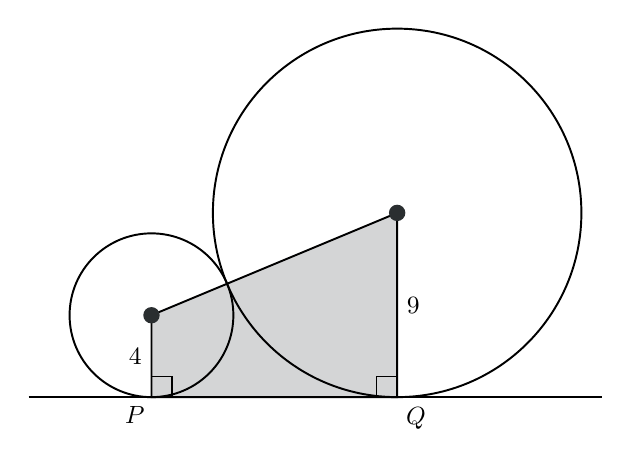
\begin{tikzpicture}[scale=0.26]
\coordinate (P) at (0,0); \coordinate (Q) at (12,0);
\coordinate (A) at (0,4); \coordinate (B) at (12,9);
\fill[ink!20] (P)--(Q)--(B)--(A)--cycle;
\draw[line width=0.7pt] (A) circle (4); \draw[line width=0.7pt] (B) circle (9);
\draw[line width=0.7pt] (-6,0)--(22,0);
\draw[line width=0.7pt] (P)--(A)--(B)--(Q)--cycle;
\draw[line width=0.5pt] (0,1)--(1,1)--(1,0); \draw[line width=0.5pt] (12,1)--(11,1)--(11,0);
\fill[ink] (A) circle (0.4); \fill[ink] (B) circle (0.4);
\node[below left,font=\small] at (P) {$P$}; \node[below right,font=\small] at (Q) {$Q$};
\node[left,font=\small] at (0,2) {4}; \node[right,font=\small] at (12,4.5) {9};
\end{tikzpicture}}\gridbox
\vfill

\noindent\pnum{22} For how many integer values of $k$ does the line $y=x+k$ intersect the circle $x^{2}+y^{2}=50$ at exactly two points?\par\vspace{2.2mm}
\hspace*{7mm}(A)\ $9$\\[1.8mm]
\hspace*{7mm}(B)\ $19$\\[1.8mm]
\hspace*{7mm}(C)\ $21$\\[1.8mm]
\hspace*{7mm}(D)\ $29$
\vfill}}
\end{textblock*}
\clearpage

\end{document}
